\documentclass[eng]{ajceam-class}
\usepackage{float}
\sloppy

% Publication Title
\title {Un enfoque basado en Redes Bayesianas Gaussianas para estudiar los efectos de la contaminación del aire en biomarcadores clínicos sanguíneos}

% Short title for the header (copy the main title if it is not too long)
\shorttitle{Redes Bayesianas Gaussianas}

% Authors
\author[1]{Joshua A. Chaidez Ochoa}
\author[1]{Luis C. Marrufo Padilla}
\author[1]{Ángel Esparza Enríquez}
\author[1]{Gustavo A. Aguilar Torreblanca}

% Author Affiliations
\affil[1]{Tecnológico de Monterrey, Escuela de Ingeniería y Ciencias, Guadalajara, Jalisco}

% Surname of the first author of the manuscript
\firstauthor{Chaidez, Marrufo, Esparza, Aguilar}

%Contact Author Information
%\contactauthor{Name A. Surname}           % Name and surname of the contact author
%\email{name.surname@email.com}            % Contact Author Email

% Publication data (will be defined in the edition)
\thisvolume{XX}
\thisnumber{XX}
\thismonth{Month}
\thisyear{20XX}

% Place your particular definitions here
\newcommand{\vect}[1]{\mathbf{#1}}  % vectors

% Insert here the abstract in English language
\abstract{La contaminación ambiental, especialmente la atmosférica, constituye uno de los grandes desafíos para la salud pública tanto en México como en el mundo, pues está asociada a diversos problemas cardiovasculares y metabólicos. Comprender cómo estos factores se relacionan es de crucial importancia para enfrentar el problema. En este estudio se propusieron, evaluaron y seleccionaron diferentes estructuras de redes bayesianas en colaboración con estudiantes y profesores de medicina. El análisis se basó en datos de la Encuesta Nacional de Salud y Nutrición 2022 y en los registros de calidad del aire reportados por la Secretaría de Medio Ambiente y Recursos Naturales en 2025. Finalmente, se utilizó el Criterio de Información Bayesiano, para seleccionar la mejor estructura aplicada a los biomarcadores. En conjunto con especialistas en salud, se determinó que una forma plausible de explicar la relación es que la concentración de contaminantes como $SO_2$, $CO$, $COV$, $PM_{10}$, $NH_3$, $PM_{2.5}$ y $NO_x$ detona procesos inflamatorios que posteriormente impactan la salud renal y cardiovascular de la población.
}

% Insert here the keywords of your work in English language
\keywords{Redes bayesianas gaussianas, contaminación atmosférica, biomarcadores, procesos inflamatorios, enfermedades cardiovasculares, salud metabólica}

% Start document
\begin{document}
\maketitle
\thispagestyle{fancy}

\section{Introducción}

 La contaminación atmosférica es una de las principales amenazas medioambientales en México. En años recientes, las ciudades han crecido rápidamente y el país se ha industrializado. Ésto provoca que la contaminación del aire alcance niveles preocupantes, no sólo en las ciudades más grandes, sino también en municipios menos urbanizados. De acuerdo a la OMS, la exposición a contaminantes por vía aérea está ligada a diversas enfermedades cardiovasculares, respiratorias y metabólicas \cite{who2024airquality}. Es de gran interés entender cómo las concentraciones altas de contaminantes afectan nuestro cuerpo y cómo es que la población mexicana está siendo afectada a causa de este problema.

En este estudio se utilizan redes bayesianas gaussianas para modelar relaciones entre variables y calcular las dependencias probabilísticas de factores sociodemográficos, marcadores biológicos y concentración de contaminantes en el aire. El objetivo es construir una red bayesiana que pueda relacionar los indicadores biológicos de la población con la exposición a diversos contaminantes del aire. Será posible entender mejor cómo estos contaminantes afectan al ciudadano promedio  mediante consultas de la red, dando una idea sobre el problema aplicado en casos específicos, lo que podría ofrecer insumos cruciales para políticas públicas y estrategias de prevención de daños.


\section{Metodología}

El análisis se realizó a partir de los datos de la Encuesta Nacional de Salud y Nutrición (ENSANUT) 2022, elaborada por el Instituto Nacional de Salud Pública \cite{ensanut2025}. Con el apoyo de dos compañeros de la Universidad Autónoma de Guadalajara (UAG), estudiantes de medicina, y de un estudiante de la Licenciatura en Químico Farmacéutico Biólogo de la Universidad Autónoma de Sinaloa (UAS), se discutieron los posibles mecanismos fisiológicos que relacionan la exposición a contaminantes del aire con la alteración en diversos biomarcadores \cite{jameson2018harrison} \cite{ross2020histologia}.

Adicionalmente, se utilizó información sobre contaminantes atmosféricos reportada por la Secretaría de Medio Ambiente y Recursos Naturales \cite{semarnat}, actualizada a junio de 2025. Entre los contaminantes considerados se incluyen:


\begin{itemize}
    \item \(\text{SO}_{2}\): dióxido de azufre  
    \item \(\text{CO}\): monóxido de carbono  
    \item \(\text{NOx}\): óxidos de nitrógeno  
    \item \(\text{COV}\): compuestos orgánicos volátiles  
    \item \(\text{PM}_{10}\): partículas con diámetro aerodinámico \(\leq 10\,\mu m\)  
    \item \(\text{PM}_{2.5}\): partículas con diámetro aerodinámico \(\leq 2.5\,\mu m\)  
    \item \(\text{NH}_{3}\): amoníaco  
\end{itemize}  

Para el análisis fue necesario integrar diferentes tablas con el fin de contar con la información requerida. En el caso de los contaminantes del aire, se asumió que los valores reportados por la SEMARNAT en 2025 son comparables con las condiciones a las que estuvieron expuestas las personas que participaron en la ENSANUT 2022; es decir, se consideraron como buenas estimaciones de la exposición a contaminantes durante 2022. 

\subsection{Construcción de las redes}

Las variables empleadas en la construcción de los DAGs fueron seleccionadas por los estudiantes de medicina y química participantes en el proyecto, considerando la relevancia fisiológica y clínica de cada una. Dichas variables incluyen:

\begin{itemize}
    \item Contaminantes atmosféricos: SO\(_2\), CO, NOx, COV, PM\(_{10}\), PM\(_{2.5}\), NH\(_3\).  
    \item Biomarcadores e indicadores de salud:  
    \begin{itemize}
        \item PC: Proteína C Reactiva  
        \item AU: Ácido úrico  
        \item I: Insulina  
        \item GS: Glucosa sérica  
        \item H: hb02, saturación de oxígeno  
        \item CL: Colesterol LDL  
        \item CH: Colesterol HDL  
        \item T: Triglicéridos  
        \item CT: Colesterol total  
        \item Cr: Creatinina  
    \end{itemize}
    \item Variable de control: E (edad)  
\end{itemize}  

A partir de estas variables se construyeron tres Diagramas Acíclicos Dirigidos (DAGs), cada uno con ligeras variaciones en las relaciones de dependencia propuestas.  

\begin{figure}[H] % 'H' fuerza a que la figura esté aquí
    \centering
    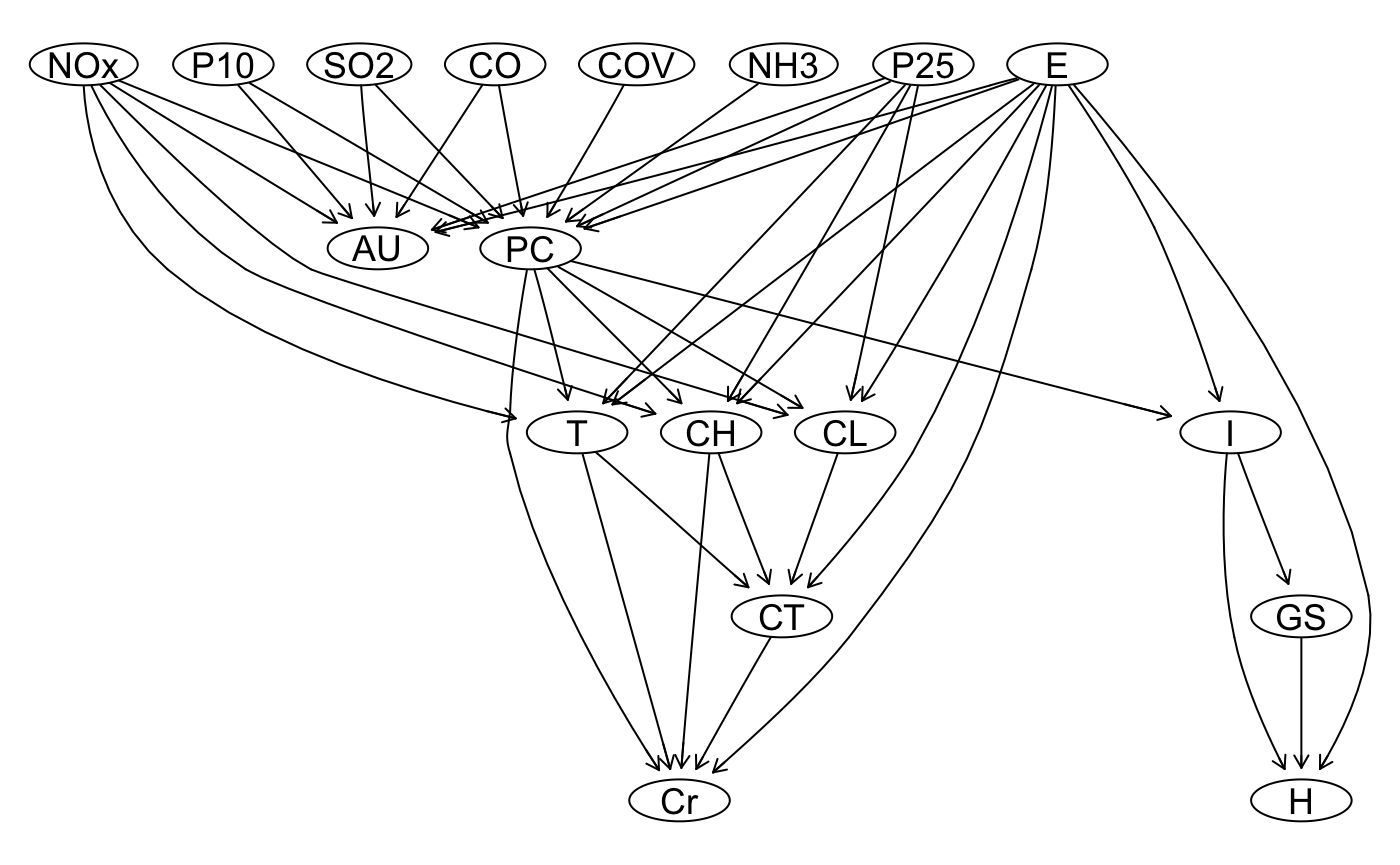
\includegraphics[width=0.5\textwidth]{dag_A.jpg}
    \caption{Estructura planteada para la DAG "A".}
    \label{fig:dag_A}
\end{figure}

En la Figura~\ref{fig:dag_A}, se modelan los contaminantes como variables exógenas que afectan directamente a la PC y al ácido úrico (AU). A partir de la PC se encadenan efectos en insulina, glucosa sérica y perfil lipídico, así como en creatinina. Este DAG enfatiza la influencia conjunta de contaminantes y edad como factor modulador.  


\begin{figure}[H] % 'H' fuerza a que la figura esté aquí
    \centering
    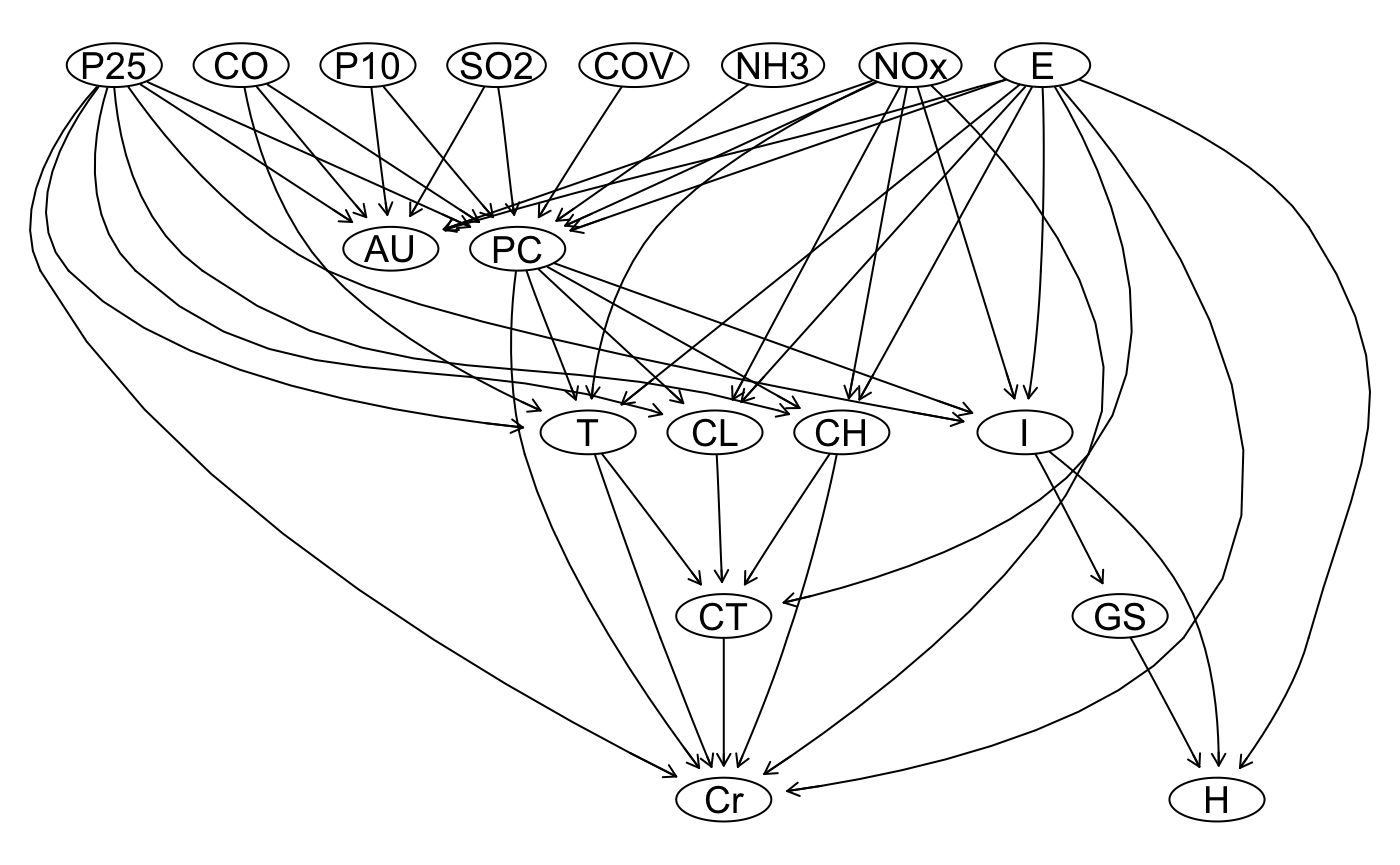
\includegraphics[width=0.5\textwidth]{dag_B.jpg}
    \caption{Estructura planteada para la DAG "B".}
    \label{fig:dag_B}
\end{figure}


En la Figura~\ref{fig:dag_B} Incorpora todos los contaminantes criterio como variables exógenas y destaca la PC como nodo central, con ramificaciones hacia el perfil lipídico, insulina y glucosa sérica. La creatinina se coloca como resultado de interacciones combinadas entre inflamación, lípidos y triglicéridos, considerando también la edad como factor de ajuste.  

\begin{figure}[H] % 'H' fuerza a que la figura esté aquí
    \centering
    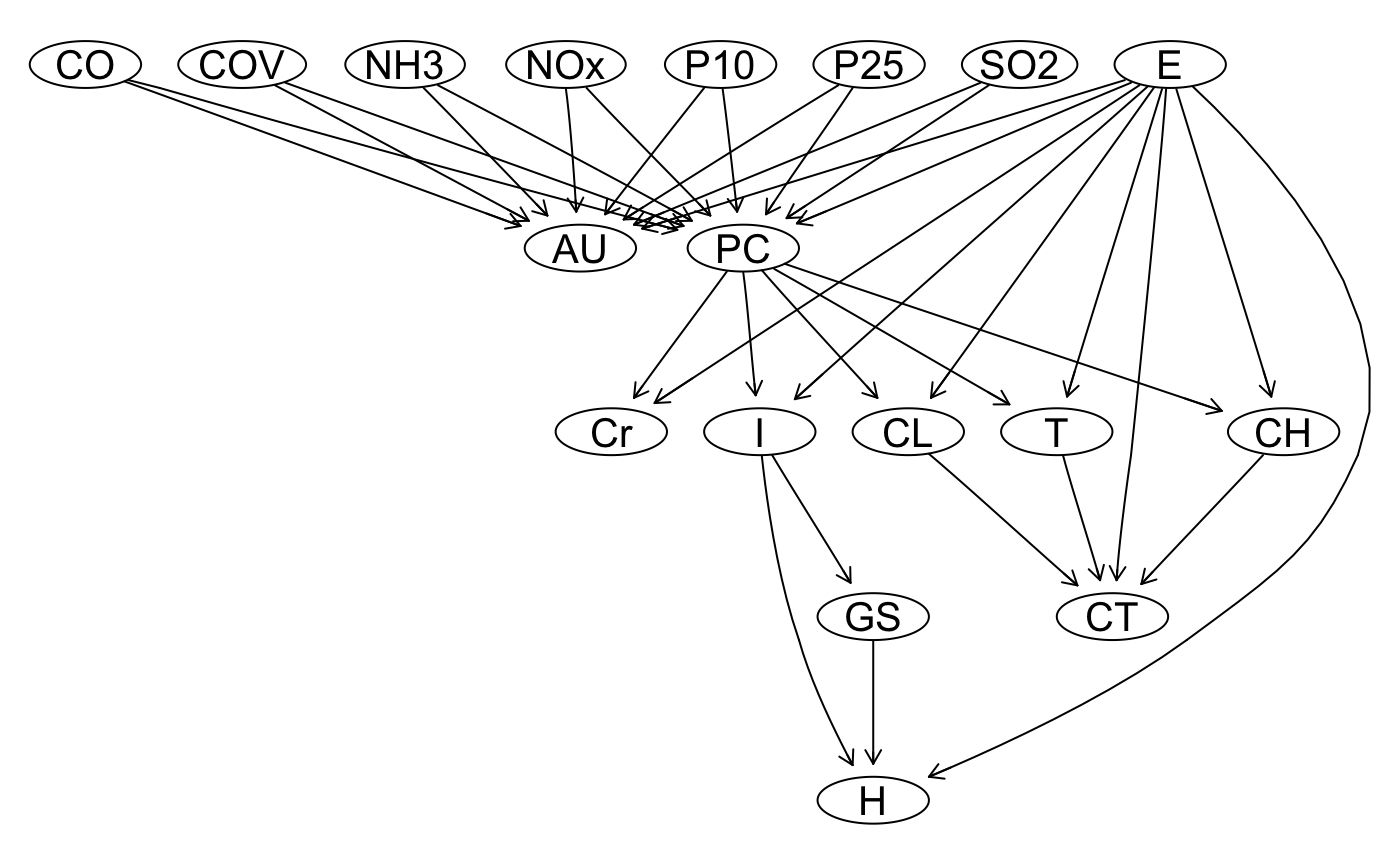
\includegraphics[width=0.5\textwidth]{dag_C.jpg}
    \caption{Estructura planteada para la DAG "C".}
    \label{fig:dag_C}
\end{figure}


Integra todos los contaminantes como entradas directas hacia PC y AU, pero concentra el resto de la red en dependencias más directas. Este DAG propone una visión más compacta de los mecanismos principales, incorporando la edad como variable de control.  

A partir de las variables contenidas en las DAGs propuestas se realizó la selección correspondiente en la base de datos de las muestras. Además, se optó por sumar todos los contaminantes por municipio con el fin de obtener una métrica concreta para cada uno. Posteriormente, se integró la base de datos de biomarcadores seleccionados con la concentración de contaminantes por municipio de cada encuestado, de modo que se trabajara con una base única que incluyera tanto los biomarcadores como la exposición individual a los contaminantes y así ajustar las DAGs propuestas a esta base de datos única.

\subsection{Selección de la DAG}

Se encontró el puntaje BIC y AIC de las redes planteadas para encontrar la red que optimizara ambos puntajes. Se muestran los puntajes obtenidos en la siguiente tabla:

\begin{table}[h!]
\centering
\resizebox{0.5\textwidth}{!}{
\begin{tabular}{|c|c|c|}
\hline
\textbf{DAG} & \textbf{Puntaje BIC} & \textbf{Puntaje AIC} \\ \hline
A        & -226004.9 & -225788.3 \\ \hline
B        & -226011.7  & -225781.0  \\ \hline
C        & -226011.7  & -225814.7  \\ \hline
\end{tabular}
}
\caption{Puntajes BIC y AIC para cada estructura DAG planteada.}
\label{tab:tabla_BIC_AIC}
\end{table}

Las redes eran muy similares y no hubo una red que optimizara ambos puntajes. Se seleccionó la estructura "A" mostrada en la Figura~\ref{fig:dag_A}, tomando como base el puntaje BIC (véase Tabla~\ref{tab:tabla_BIC_AIC}). Aunque otras configuraciones mostraron ligeras ventajas en criterios como el AIC, un mayor puntaje en el BIC indica una mayor parsimonia y menor riesgo de sobreajuste. Ésto resulta especialmente relevante para la etapa de consultas, ya que una red con menos arcos tiende a generar inferencias más estables, interpretables y robustas frente a la variabilidad de los datos, favoreciendo la coherencia de las probabilidades condicionales obtenidas. De esta forma, se privilegia la claridad y la validez de los resultados sobre una ganancia marginal en ajuste predictivo.


\subsection{Agregando variables categóricas}

A la red seleccionada (vea Figura~\ref{fig:dag_A}) le agregamos las variables categóricas que son el sexo y el estrato. Estas variables no fueron agregadas en un principio ya que forman una red mixta entre variables discretas y continuas y no habrían permitido el uso de los puntajes BIC y AIC para comparar el desempeño de las redes. A continuación se muestra la nueva estructura:

\begin{figure}[H] % 'H' fuerza a que la figura esté aquí
    \centering
    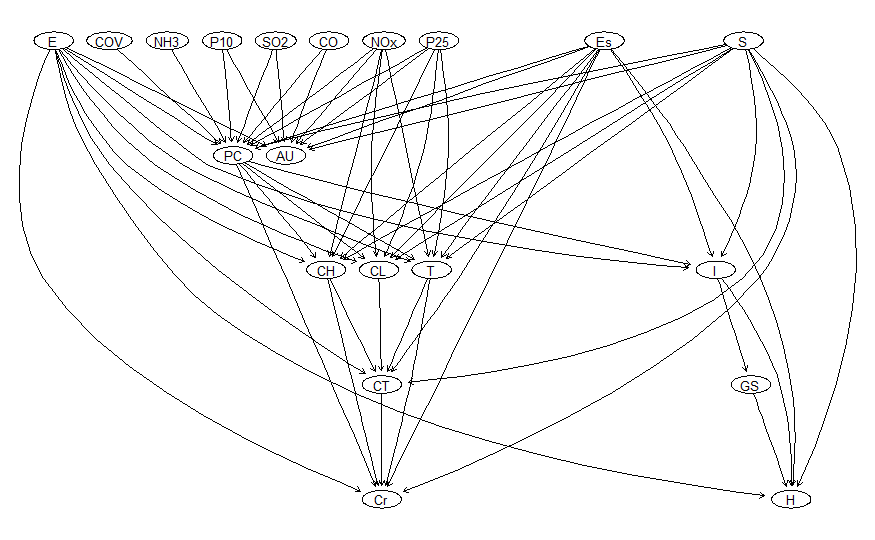
\includegraphics[width=0.5\textwidth]{dag_SE.png}
    \caption{Estructura de la DAG "A" (vea Figura~\ref{fig:dag_A}) incluyendo las variables categóricas \texttt{sexo} y \texttt{estrato}.}
    \label{fig:dag_Ex}
\end{figure}
Al agregar manualmente las variables sexo y estrato, la red captura diferencias demográficas y contextuales que influyen en las relaciones entre contaminación y biomarcadores. El sexo refleja posibles variaciones fisiológicas (p. ej., en metabolismo de glucosa), mientras que el estrato representa el entorno (rural, urbano, metropolitano) y su efecto sobre la exposición. Con esto, las consultas pueden considerar no sólo contaminantes, sino también características poblacionales relevantes.


\section{Resultados}
Se le realizaron las siguientes consultas a la red con ayuda de los estudiantes del área:

\begin{itemize}
    \item ¿Cuál es la probabilidad de presentar inflamación clínicamente relevante (PC $\geq 1$ mg/L) en una mujer de 45 años de zona metropolitana con exposición a PM$_{2.5} = 30$ y $NO_x = 40$?  
    
    $P(PC \geq 1 \mid (S = mujer, PM_{2.5} = 30, NO_x = 40, E = 45, Es = zona$ $metropolitana)) = 0.3121$
    
    \item ¿Cuál es la probabilidad de tener triglicéridos $\geq 150$ mg/dL en un hombre de 55 años que vive en zona urbana con PM$_{2.5} = 25$ y $NO_x = 35$?  
    
    $P(T \geq 150 \mid (S = hombre, PM_{2.5} = 25, NO_x = 35, E = 55, Es = zona$ $urbana)) = 0.5996$
    
    \item ¿Cuál es la probabilidad de tener HDL bajo (<40 mg/dL en hombres, <50 en mujeres) en una mujer de 50 años en zona rural con PM$_{2.5}$ y $NO_x$ altos?  
    
    $P(CH < 50 \mid (S = mujer, PM_{2.5} \text{ alto}, NO_x \text{ alto}, E = 50, Es = zona$ $rural)) = 0.8083$
\end{itemize}

\subsection{Consideraciones adicionales}

Otro aspecto a tomar en cuenta en nuestra red es la inclusión de modelos no paramétricos. Dependiendo de si pueden mejorar los resultados de ajuste como el BIC y AIC. Tal como señalan Koller y Friedman \cite{koller2009pgm}, los modelos gaussianos son útiles y confiables, pero imponen supuestos muy limitantes a la linealidad y normalidad en las distribuciones. Estos supuestos suelen ser una simplificación alterna demasiado excesiva para la realidad, ya que muchas variables ambientales y biológicas presentan asimetrías, colas pesadas e incluso relaciones no lineales. Dado esto, al explorar modelos no paramétricos es posible capturar de forma más fiel cómo se distribuyen los datos, dando así un mejor ajuste y puntajes más favorables de BIC y AIC.

En esta investigación, la medición con los modelos no paramétricos si mejoró el BIC, teniendo un resultado de $-225696$, a comparación de la DAG mostrada en la Figura~\ref{fig:dag_Ex} de $-226004.9$, demostrando el punto de la investigación.

\section{Conclusiones}
Los resultados obtenidos mediante las consultas a la red final permiten demostrar que las dependencias probabilísticas, junto con una estructura de red bien definida y respaldada por información médica, pueden reflejar la relación entre las variables, incluso tratándose de un fenómeno tan complejo como la biología. Además, constituyen una herramienta útil para simular resultados clínicos plausibles.

En general, todas las DAGs planteadas muestran una relación clara entre los factores ambientales y los biomarcadores. La exposición a la contaminación ambiental detona procesos inflamatorios vinculados con el valor de la proteína C reactiva (PC) en sangre. A partir de ahí se establece la conexión con otros biomarcadores, como la insulina, que finalmente contribuyen al deterioro del sistema cardiovascular y del metabolismo. Esta información resulta útil porque permite comprender de manera más profunda cómo los contaminantes afectan la salud de la población, y puede servir de base tanto para la formulación de nuevas leyes de salud pública como para reforzar la justificación de políticas orientadas a reducir la contaminación en nuestras ciudades. Sin embargo, es necesario reconocer cómo se obtuvo la información y cuáles son las limitaciones del estudio.

Entre los principales problemas relacionados con la precisión, destaca el uso de datos de contaminantes atmosféricos del año 2025 frente a muestras biológicas de 2022, lo que podría afectar la validez de las asociaciones identificadas. Además, aunque el análisis de la relación entre factores ambientales y biológicos se realizó en colaboración con estudiantes y profesores del área de salud, sigue siendo relativamente básico y superficial, ya que posiblemente no se consideraron otros procesos biológicos relevantes para un diagnóstico más integral. En una versión futura del estudio sería recomendable incluir un mayor número de parámetros médicos y realizar un análisis más exhaustivo de los procesos biológicos vinculados con estas afectaciones.


% Include references
\insertbibliography{References}

\end{document}
